\documentclass[tikz, border=5mm]{standalone}
\usepackage{pgfplots}
\pgfplotsset{compat=1.18}
\usetikzlibrary{calc, arrows.meta}

\begin{document}
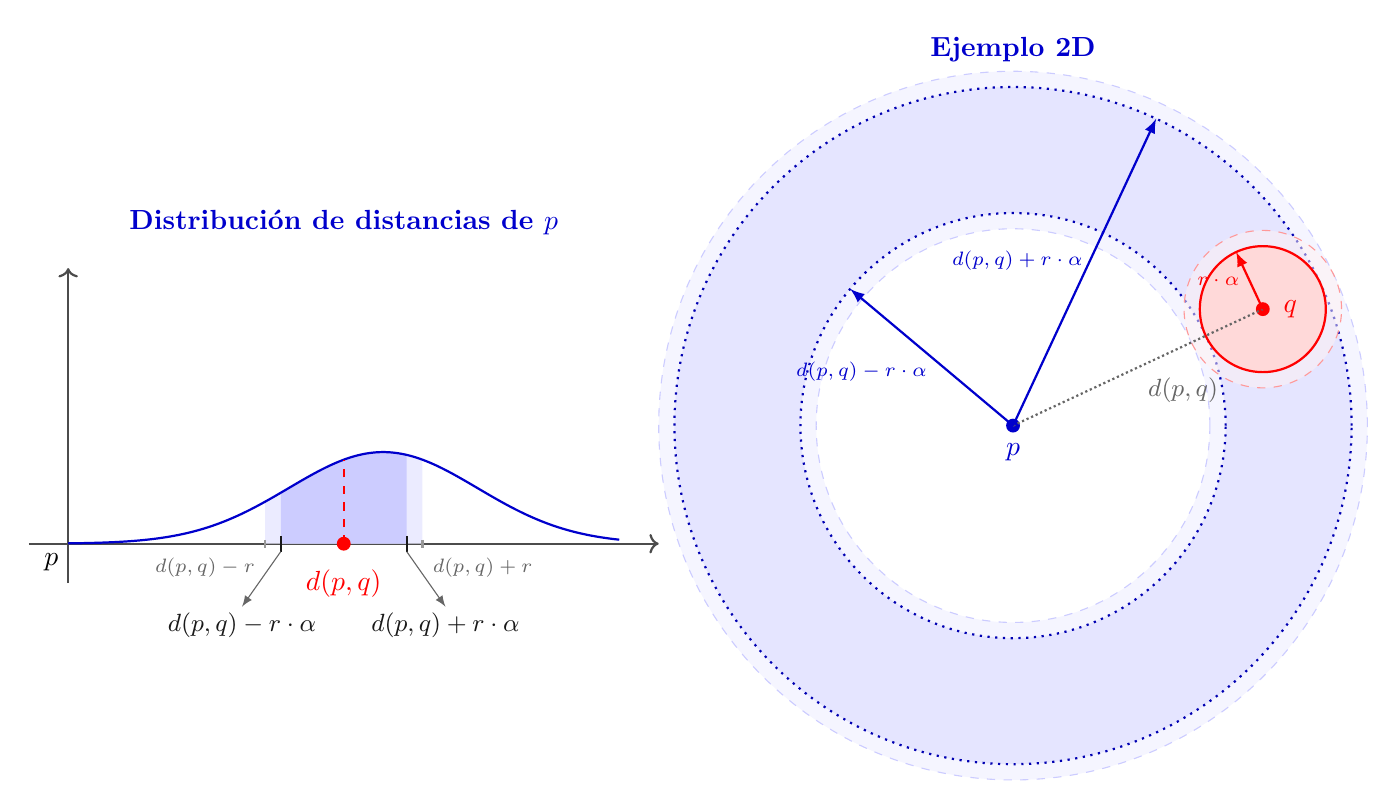
\begin{tikzpicture}

    % --- Parámetros matemáticos globales ---
    \def\dpq{3.5}       % Distancia exacta entre p y q: d(p,q)
    \def\rad{1.0}       % Radio original de la consulta q: r (incrementado a 1.0 para mejor contraste)
    \def\alphaFactor{0.8} % Factor alfa para el rango reducido

    % Límites Originales (alpha = 1.0)
    \def\rminOne{\dpq-\rad}
    \def\rmaxOne{\dpq+\rad}

    % Límites Reducidos (alpha = 0.8)
    \def\rminAlpha{\dpq-\rad*\alphaFactor}
    \def\rmaxAlpha{\dpq+\rad*\alphaFactor}
    
    \def\muP{4.0}       % Media de la gaussiana
    \def\sigmaP{1.2}    % Desviación estándar de la gaussiana

    % Función gaussiana escalada
    \tikzset{
        declare function={
            gauss(\x,\mu,\sigma)=3.5 * (1/(\sigma*sqrt(2*pi))*exp(-((\x-\mu)^2)/(2*\sigma^2)));
        }
    }

    % =========================================================================
    % PARTE IZQUIERDA: Distribución de distancias relativas al pivote p (1D)
    % =========================================================================
    \begin{scope}[xshift=0cm]
        
        % Ejes
        \draw[->, thick, black!70] (-0.5, 0) -- (7.5, 0) node[right] { };
        \draw[->, thick, black!70] (0, -0.5) -- (0, 3.5) node[above] { };
        \node[below left] at (0,0) {$p$};

        % 1. Sombrear rango original (alpha = 1) - Azul muy tenue
        \fill[blue!8] (\rminOne, 0) 
            -- plot[domain=\rminOne:\rmaxOne, samples=50] (\x, {gauss(\x,\muP,\sigmaP)}) 
            -- (\rmaxOne, 0) -- cycle;

        % 2. Sombrear rango acotado (alpha = 0.8) - Azul más intenso
        \fill[blue!20] (\rminAlpha, 0) 
            -- plot[domain=\rminAlpha:\rmaxAlpha, samples=50] (\x, {gauss(\x,\muP,\sigmaP)}) 
            -- (\rmaxAlpha, 0) -- cycle;

        % 3. Dibujar la curva gaussiana principal
        \draw[thick, blue!80!black, smooth, domain=0:7, samples=100] plot (\x, {gauss(\x,\muP,\sigmaP)});

        % 4. Línea de la distancia d(p,q) exacta
        \draw[red, thick, dashed] (\dpq, 0) -- (\dpq, {gauss(\dpq,\muP,\sigmaP)});
        \fill[red] (\dpq, 0) circle (2.5pt) node[below=6pt, font=\bfseries] {$d(p,q)$};

        % 5. Marcar límites originales (alpha = 1) en la parte inferior
        \draw[thick, black!40] (\rminOne, 0.05) -- (\rminOne, -0.05) node[below left, font=\scriptsize, color=black!60] {$d(p,q)-r$};
        \draw[thick, black!40] (\rmaxOne, 0.05) -- (\rmaxOne, -0.05) node[below right, font=\scriptsize, color=black!60] {$d(p,q)+r$};

        % 6. Marcar límites reducidos (alpha = 0.8) con indicadores más altos
        %\draw[thick, black!90] (\rminAlpha, 0.1) -- (\rminAlpha, -0.1) node[below, xshift=-8pt, yshift=-16pt, font=\small\bfseries] {$d(p,q)-r\cdot\alpha$};
        %\draw[thick, black!90] (\rmaxAlpha, 0.1) -- (\rmaxAlpha, -0.1) node[below, xshift=8pt, yshift=-16pt, font=\small\bfseries] {$d(p,q)+r\cdot\alpha$};

        %---
        
        % 6. Marcar límites reducidos (alpha = 0.8) con líneas indicadoras a sus leyendas
        % Límite izquierdo (Contracción inferior)
        \draw[thick, black!90] (\rminAlpha, 0.1) -- (\rminAlpha, -0.1); % Marca en el eje
        \draw[transparent] (\rminAlpha, -0.1) -- (\rminAlpha, -0.8) 
            node[below, black!90, font=\small\bfseries, opaque, fill=white, inner sep=2pt, xshift=-14pt] (lblMin) {$d(p,q)-r\cdot\alpha$};
        \draw[thin, black!60, ->, >=latex] (\rminAlpha, -0.1) -- (lblMin.north); % Línea indicadora recta

        % Límite derecho (Contracción superior)
        \draw[thick, black!90] (\rmaxAlpha, 0.1) -- (\rmaxAlpha, -0.1); % Marca en el eje
        \draw[transparent] (\rmaxAlpha, -0.1) -- (\rmaxAlpha, -0.8) 
            node[below, black!90, font=\small\bfseries, opaque, fill=white, inner sep=2pt, xshift=+14pt] (lblMax) {$d(p,q)+r\cdot\alpha$};
        \draw[thin, black!60, ->, >=latex] (\rmaxAlpha, -0.1) -- (lblMax.north); % Línea indicadora recta
        %---
        % Flechas de contracción visual en el eje X
        %\draw[-{Stealth}, thick, blue!70!black] (\rminOne, -0.5) -- (\rminAlpha, -0.5) node[midway, above, font=\tiny] {$\alpha$};
        %\draw[-{Stealth}, thick, blue!70!black] (\rmaxOne, -0.5) -- (\rmaxAlpha, -0.5) node[midway, above, font=\tiny] {$\alpha$};

        % Título
        \node[above, font=\bfseries, blue!80!black] at (3.5, 3.8) {Distribución de distancias de $p$};
        
    \end{scope}


    % =========================================================================
    % PARTE DERECHA: Vista espacial geométrica (2D)
    % =========================================================================
    \begin{scope}[xshift=12cm, yshift=1.5cm]
        
        \coordinate (P) at (0,0);
        \coordinate (Q) at (25:\dpq);

        % 1. Anillo Original (\alpha = 1.0) - Sutil
        \fill[blue!4, even odd rule] (P) circle (\rmaxOne) (P) circle (\rminOne);
        \draw[blue!20, dashed] (P) circle (\rminOne);
        \draw[blue!20, dashed] (P) circle (\rmaxOne);

        % 2. Anillo Acotado (\alpha = 0.8) - Más visible
        \fill[blue!10, even odd rule] (P) circle (\rmaxAlpha) (P) circle (\rminAlpha);
        \draw[blue!70!black, thick, dotted] (P) circle (\rminAlpha);
        \draw[blue!70!black, thick, dotted] (P) circle (\rmaxAlpha);

        % 3. Bola de consulta original (r) y bola reducida (r * \alpha)
        \fill[red!5, fill opacity=0.5] (Q) circle (\rad);
        \draw[red!40, dashed] (Q) circle (\rad); % Frontera original r
        
        \fill[red!15] (Q) circle (\rad*\alphaFactor);
        \draw[red, thick] (Q) circle (\rad*\alphaFactor); % Frontera acotada r * alpha

        % 4. Marcar centros
        \fill[blue!80!black] (P) circle (2.5pt) node[below=3pt, font=\bfseries] {$p$};
        \fill[red] (Q) circle (2.5pt) node[right=4pt, font=\bfseries] {$q$};

        % 5. Vectores y etiquetas de distancia
        \draw[thick, densely dotted, black!60] (P) -- (Q) node[midway, below right, font=\small] {$d(p,q)$};
        
        % Vector del radio acotado
        \draw[red, ->, >=latex, thick] (Q) -- ++(115:\rad*\alphaFactor) node[midway, left, font=\scriptsize] {$r\cdot\alpha$};
        
        % Radios del anillo acotado (alpha = 0.8)
        \draw[blue!80!black, ->, >=latex, thick] (P) -- (140:\rminAlpha) node[midway, below left=-2pt, font=\scriptsize] {$d(p,q)-r\cdot\alpha$};
        \draw[blue!80!black, ->, >=latex, thick] (P) -- (65:\rmaxAlpha) node[midway, above left=-3pt, font=\scriptsize] {$d(p,q)+r\cdot\alpha$};

        % Título
        \node[above, font=\bfseries, blue!80!black] at (0, 4.5) {Ejemplo 2D};

    \end{scope}

    % Línea divisoria
    %\draw[thick, gray!20, dashed] (8.5, -1.8) -- (8.5, 6.0);

\end{tikzpicture}
\end{document}